\chapter{Funciones}

\lettrine[lines=2]{C}{ecilia y Antonia} volvieron a enfrentarse al día
siguiente a la computadora, dócil receptora de sus textos.

---Muy bien ---esta vez fue Cecilia quien empezó---; las relaciones
matemáticas entre horas y grados para ambos he\-mis\-fe\-rios no son
difíciles de lograr ---y tras garrapatear unos instantes sobre uno de
los tantos papeles que llenaban de confusión el escritorio de Antonia,
presentó dichas funciones:
\begin{subequations}
\begin{align}
      G_{\text{sur}}(H) &= 270^{\circ} - 15^{\circ} \times H \label{eq:formula-hora-a-grados-sur}\\
      G_{\text{norte}}(H) &= 15^{\circ} \times H - 90^{\circ} \label{eq:formula-hora-a-grados-norte}
\end{align}
\end{subequations}
\label{eq:formula-hora-a-grados}
\guillemotright $H$ es el valor de la hora que queremos transformar en
grados; $G_{\text{sur}}(H)$ y $G_{\text{norte}}(H)$ son las funciones
que realizan dicha transformación para ambos hemisferios ---aclaró
Cecilia.

---¿Te molesta si compruebo la veracidad de tus relaciones probándolas
con algunos valores particulares? ---pre\-gun\-tó Antonia procurando con
un tono neutro disimular su intención de molestar a su amiga.

Cecilia, por su parte, no pudo esconder su contrariedad:

---Por supuesto que no; dale, adelante ---dijo, mientras se recostaba
con cierta brusquedad contra el respaldo de la silla.

---A ver... Veamos... ---musitó Antonia mientras escribía sobre el
mismo pedazo de papel---. Si uso la ecuación
\ref{eq:formula-hora-a-grados-sur} con las horas 6, 9, 12, 15 y 18,
obtengo... ---y tras unos momentos en los que aprovechó los últimos
rincones del ya atestado papel, confirmó---: Sí, perfecto: me da
180$^{\circ}$, 135$^{\circ}$, 90$^{\circ}$, 45$^{\circ}$ y
0$^{\circ}$, tal como debe ser.\footnote{El hecho de que la fórmula
  funcione para cinco valores particulares no garantiza su eficacia
  para todo el conjunto continuo que abarca las 12 horas que van de
  las 6:00 a las 18:00. (Nota del Editor)}$^,$\footnote{¡Sos cabeza
  dura, eh! (Nota de Antonia, Cecilia y Luis)}

---¿No querés confirmar también la eficacia de la fórmula
\ref{eq:formula-hora-a-grados-norte}? ---soltó Cecilia con una
sonrisa quebrada que podía tomarse como un desafío.

---No hace falta ---admitió Antonia, sa\-tis\-fe\-cha---. Estoy segura
de que está bien. Ahora lo que tenemos que hacer es escribirlas en el
lenguaje de \openscad.

\section[function]{\lstinline!function!}

---Para escribir una función usamos la expresión \lstinline!function!
---di\-jo Antonia, mientras tomaba el teclado.

\begin{lstlisting}[numbers=none]
function suma(a,b)=a+b;
\end{lstlisting}

\guillemotright Como podés apreciar, la sintaxis es bastante intuitiva
---An\-to\-nia, una vez más, confundía deseo con realidad---. La palabra
\lstinline!function! es seguida por el nombre que queremos darle a la
función; en este caso `\lstinline!suma!'. Al nombre le siguen,
encerrados entre paréntesis, los parámetros que dicha función admitirá
y sobre los que va a operar. A continuación, y tras un signo `=',
sigue la expresión que devolverá la función como valor.

A Cecilia no le parecía insensato lo que Antonia le contaba, pero
sentía que sólo unos ejemplos le darían la seguridad que necesitaba
para entender un giro lingüístico nuevo.

---En la descripción de cualquier nuevo objeto, la invocación a la
función vale tanto como el resultado que devuelve; mirá ---siguió
Antonia:

    \begin{lstlisting}[numbers=none]
cube([suma(1,1),suma(2,2),suma(-2,3)]);
    \end{lstlisting}

    \begin{figure}[ht]
      \centering
      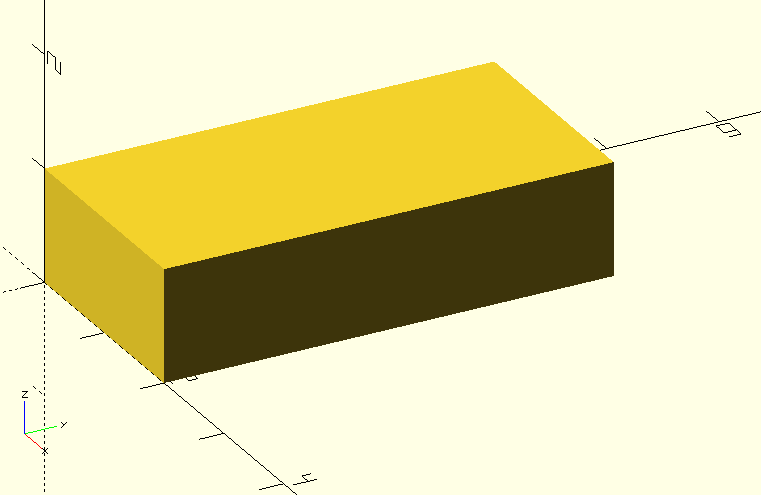
\includegraphics[width=.45\textwidth]{imagenes/cubo-funcion}      
      \caption[Cubo (función)]{Cubo cuyos lados son calculados por una
        función.}
      \label{fig:cubo-funcion}
    \end{figure}


    Cecilia pensó que se trataba de una forma muy rebuscada de
    escribir \lstinline!cube([2,4,1])!, pero captó la idea; además, ya
    estaba acostumbrada a los ejemplos triviales de Antonia.

    ---Por supuesto, este ejemplo es bastante tonto ---re\-co\-no\-ció
    su amiga---. Uno que me gusta mucho es éste:

    \begin{lstlisting}
function elipse_cartesiana(a,e,theta)=
  let(b=a*sqrt(1-e*e), 
      x=a*cos(theta),
      y=b*sin(theta))
    [x,y];
    \end{lstlisting}

   Cecilia volvió a sentir en el cuerpo ese vértigo feliz que le
   producía un misterio en el que se presentía con claridad un orden
   secreto.

   ---En una función también podés declarar variables auxiliares
   ---dijo Antonia---, pero debés hacerlo con la palabra clave
   \lstinline!let!, que recibe entre paréntesis dichas variables junto
   con su definición. En esta función en particular, quiero calcular
   las coordenadas cartesianas $x$ e $y$ del punto de una elipse de la
   que conozco su semieje mayor ($a$) y excenticidad ($e$), para un
   cierto ángulo $\theta$.

   \guillemotright En la líneas 2 a 4 de la función
   \lstinline!elipse_cartesiana! calculo tres variables dentro de un
   \lstinline!let!: \texttt{b}, \texttt{x} e \texttt{y}. Las tres,
   como te conté, deben ir dentro de un par de paréntesis, y separadas
   unas de otras mediante comas. Finalmente, en la línea 5 indico el
   resultado que debe devolver la función: el vector \texttt{[x,y]},
   con las coordenadas buscadas.

   \begin{figure}[ht]
     \centering
       \begin{tikzpicture}[scale=.6]

    \pgfmathsetmacro{\a}{4} 
    \pgfmathsetmacro{\e}{0.7}     
    \pgfmathsetmacro{\b}{\a * sqrt(1-\e*\e)}
    \pgfmathsetmacro{\rt}{0.2};
    \pgfmathsetmacro{\rs}{0.4};
    \pgfmathsetmacro{\alfa}{30};
    

%    \clip (-\a*.08,-\a*.08) rectangle (\a*.08,\a*.08);
    
    \coordinate (O) at (0,0);
    \coordinate (T) at ({\a*cos(\alfa)},{\b*sin(\alfa)}); % Tierra
    \coordinate (x) at ($(0,0)!(T)!(\a,0)$);
    \coordinate (y) at ($(0,0)!(T)!(0,\a)$);

    \draw[very thick] (0,0) ellipse [x radius=\a, y radius=\b];

    \draw[dashed, thick] (0,0) --   (\a,0);

    \draw[thin, decoration={brace, mirror, raise=5pt, amplitude=5pt},
    decorate] (0,0) -- node [below=10pt] { $a$} (\a,0);
  
    \draw[dashed, thick] (0,\b) --  (0,0);

    \draw[thin, decoration={brace, raise=5pt, amplitude=5pt, mirror},
    decorate] (0,\b) -- node [left=10pt] { $b$} (0,0);

    \filldraw (T) circle (2pt);

    \draw[dotted, thick] (T) -- (x);
    \draw[dotted, thick] (T) -- (y);

    \draw[thin, decoration={brace, raise=5pt, amplitude=5pt,aspect=.4},
    decorate] (y) -- node [above=10pt,pos=.4] { $x$} (T);

    \draw[thin, decoration={brace, raise=12pt, amplitude=5pt, mirror},
    decorate] (x) -- node [right=16pt] { $y$} (T);
   
    \draw pic [draw=green!80!black, fill=green!20, angle
     radius=1.6cm, angle eccentricity=.7, "$\theta$", opacity=.7]
     {angle = x--O--T};

     \draw (O) -- (T);
  
  \end{tikzpicture}
     \caption{Elipse}
     \label{fig:elipse}
   \end{figure}

   Cecilia procuró traer a su memoria viejos recuerdos geométricos,
   para lo cual le resultó muy útil la figura \ref{fig:elipse}: para
   toda elipse se verificaba la siguiente relación entre $a$, $b$ (el
   semieje menor) y $e$:
   \[b=a\times(1-e^2)\]
   y $x$ e $y$ podían expresarse como
\[ \left\{
    \begin{aligned}
      x&=a\times \cos \theta\\
      y&=b\times \sen \theta
    \end{aligned} \right.
\]

---Una función puede devolver cualquier tipo de valor ---ex\-pli\-có
Antonia---; ésta en particular devuelve \lstinline![x,y]!: un vector
cuyos elementos son $x$ e $y$. Ahora podemos usarla para escribir, por
ejemplo, una elipse de esferas:

    \begin{lstlisting}
module elipse(a,e,grosor,n_esferas=100){
  for(i=[0:n_esferas-1]){
    theta=i*360/n_esferas;
    pos=elipse_cartesiana(a,e,theta);
    translate([pos.x,pos.y,0])
      sphere(r=grosor);
  }
}
elipse(100,.7,5);
    \end{lstlisting}

    \begin{figure}[ht]
      \centering
      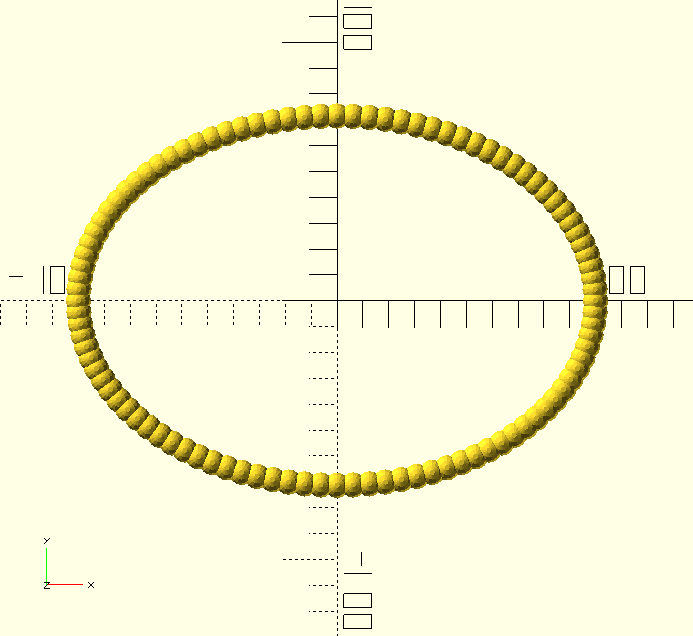
\includegraphics[width=.5\textwidth]{imagenes/elipse-funcion}
      \caption{Elipse producida por Antonia con una función.}
      \label{fig:elipse-funcion}
    \end{figure}


    \guillemotright La línea clave es la 4: en ella se calculan las
    coordenadas de cada esfera gracias a la función que escribí antes,
    y se guardan en la variable \lstinline!pos!  ---desarrolló
    Antonia---. Luego, en la línea 5, rescato esas coordenadas con
    \lstinline!pos.x! y \lstinline!pos.y! para efectuar la debida
    traslación de cada esfera del perímetro de la elipse.

    Cecilia no parecía muy convencida:

    ---A ver... ¿me dejás probrar algo? ---y sin esperar respuesta,
    tomó el teclado para sí.

   
    \begin{lstlisting}
module elipse_bis(a,e,grosor,n_esferas=100){
  for(i=[0:n_esferas-1]){
    theta=i*360/n_esferas;
    b=a*sqrt(1-e*e);
    x=a*cos(theta);
    y=b*sin(theta);
    translate([x,y,0])
      sphere(r=grosor);
  }
}
elipse_bis(100,.7,5);
\end{lstlisting}

\begin{figure}[ht]
  \centering
  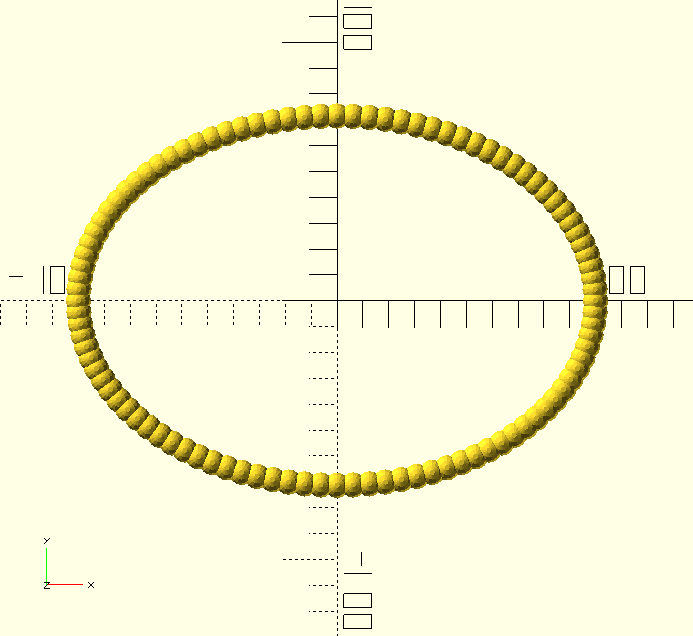
\includegraphics[width=.5\textwidth]{imagenes/elipse-funcion}
  \caption{Elipse producida por Cecilia sin usar una función.}
  \label{fig:elipse-funcion-2}
\end{figure}

Cecilia dirigió a Antonia una mirada de interrogación, al tiempo que
señalaba el resultado de la figura \ref{fig:elipse-funcion-2}:

---¿Qué onda? ¿No se podía hacer así?

---Sí, por supuesto ---admitió su amiga---. En principio, puede
argumentarse que se trata de una cuestión de gustos. Personalmente,
cuando detecto que una serie de cálculos merece ser `aislada', la
encierro en una función propia.

Antonia comprendió que como justificación era muy pobre, y hasta
injusta respecto de las dilatadas posibilidades expresivas de las
funciones. Tras un instante y un inevitable suspiro, trató de
mejorarla:

---A medida que una escribe advierte que hay ciertas costumbres o
vicios en los que caemos una y otra vez, y que suelen desencadenar los
mismos nefastos resultados: uno de ellos es encargar a un solo bloque
de texto (un módulo, por ejemplo) demasiada `responsabilidad' o
`trabajo'. Cuando eso pasa, y detectás un error luego (a veces,
cientos de líneas más tarde), te encontrás sumergida en ese viejo
bloque de texto tratando de encontrar en qué línea está el
problema. Pero si en lugar de eso vos repartís el trabajo en bloques
mínimos, responsables cada uno de una tarea elemental y bien definida,
cualquier revisión posterior (¡e inevitable!) será sensiblemente más
fácil.

A Cecilia le pareció razonable lo que le confió Antonia, aunque no
terminaba de comprenderlo del todo. Pensó que quizá lo mejor sería
intentar seguir su consejo, pero sin adoptarlo como una regla rígida
que la entumeciera en su proceso de escritura.

---Además ---abundó Antonia---, imaginate que más tarde te das cuenta
de que hay una forma más eficiente o rápida de calcular el mismo
valor: ¡deberías modificar cada aparición de esas fórmulas en cada
módulo que las empleara!  ---Antonia abrió grandes los ojos y separó
sus brazos, como si los gestos constituyeran un argumento: otro
defecto más de su condición docente. A Cecilia esta razón le gustó un
poco más; en cualquier caso, y para no seguir tolerando otra de las
interminables apologías de su amiga, decidió lanzarse a la escritura
de...

\section{Las fórmulas del ángulo}

---Entonces nuestras fórmulas podrían quedar... ¿así?  ---pre\-gun\-tó
Cecilia, mientras escribía rápidamente.

\begin{lstlisting}
function alfa_sur(hora)=270-15*hora; 
function alfa_norte(hora)=15*hora-90;
\end{lstlisting}

---Exacto ---confirmó Antonia con una sonrisa.

\section[echo]{\lstinline!echo!}

---Yo, cuando escribo, no puedo liberarme de una incómoda sensación
---con\-fe\-só Antonia---: aún cuando me encuentro segura de que lo
que acabo de escribir es correcto, necesito verificarlo con ejemplos
concretos. ¡Ay! ¡Si supieras la de sorpresas que me deparó el uso
incomprobado de algunos de mis párrafos..!

Cecilia pensó que Antonia había caído en otra de sus exageraciones
retóricas; pero la dejó continuar.

---Una sentencia que me resulta muy útil a fin de conjurar esas
contrariedades es \lstinline!echo!: imprime en la consola lo que
recibe entre paréntesis ---y Antonia tecleó con rapidez algunos
ejemplos tontos.

\begin{lstlisting}
echo(1);
echo(1+1);
echo("Antonia y Cecilia son", 18/9, "amigas inseparables.");
\end{lstlisting}


\begin{figure}[ht]
  \centering
  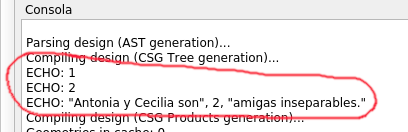
\includegraphics[width=.8\textwidth]{imagenes/consola-echo-1}  
  \caption{Antonia ilustra el uso de la instrucción \lstinline!echo!.}
  \label{fig:consola-echo-1}
\end{figure}


\guillemotright Ahora podemos confirmar que nuestras funciones
funcionan.  ---Antonia no podía evitar esos juegos de palabra ñoños.

    \begin{lstlisting}
for(h=[6:3:18])
  echo(h,alfa_sur(h),alfa_norte(h));
\end{lstlisting}

\begin{figure}[ht]
  \centering
  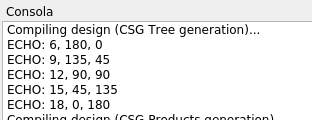
\includegraphics[width=.6\textwidth]{imagenes/consola-echo-funciones}
       \caption[Comprobación de funciones con
       \lstinline!echo!]{Antonia comprueba las funciones que calculan
         el ángulo $\alpha$.}
  \label{fig:consola-echo-funciones}
\end{figure}
  


Cecilia se irguió en su silla, entusiasmada:

---¡Está bueno!  ---tuvo que reconocer ante la figura
\ref{fig:consola-echo-funciones}.

\section{Condicionales en funciones}

---Ahora ya podríamos usar esas funciones dentro de nuestros
generadores de dígitos, para darles la dirección adecuada en función
de la hora y el hemisferio en el que el usuario se encuentra.
---An\-to\-nia se detuvo, suspendiendo el último punto en el aire.

Cecilia entendió que eso y el uso del modo potencial estaban
sugiriendo que ésa no era la solución que su amiga consideraba
óptima. Decidió seguirle el juego:

---Peerooo.... ---arrastró, invitándola a seguir.

Antonia sonrió al ver adivinada su intención:

---¿No sería más lindo que el módulo \lstinline!digito! simplemente
confiara en el resultado que le brinde una suerte de función
\lstinline!alfa(H)!, la cual estaría a cargo de decidir qué ángulo
ofrecer dependiendo del hemisferio..? ¿Acaso vamos a agregar a las
obligaciones de \lstinline!digito! la de indagar qué función usar..?

Cecilia ya estaba demasiado cansada como para disentir. Además, debía
admitir que la idea, en principio, sonaba bien; con un movimiento de
cabeza, asintió.

---Bien ---aprobó Antonia con una sonrisa, aparentemente satisfecha de
su capacidad de persuasión---. Entonces vamos a crear una variable con
la que el usuario pueda definir el hemisferio para el cual quiere
construir su reloj, y una función \lstinline!alfa(H)! que utilice
\lstinline!alfa_sur(H)!  o a \lstinline!alfa_norte(H)! dependiendo del
valor de aquella ---y con entusiasmo volvió a sacar ligeros chasquidos
del ya fatigado teclado.


\begin{lstlisting}
hemisferio="sur";

function alfa(hora)=
  hemisferio=="sur" ? alfa_sur(hora) : alfa_norte(hora);
\end{lstlisting}

Cecilia volvió a erguirse en su silla:

---¡Epa!  ---exclamó---. ¿Qué es eso?

---Es la forma en que se escriben las estructuras condicionales en las
funciones ---declaró Antonia, quien disfrutaba sensiblemente
provocando la perplejidad en su amiga---. En las mismas no se puede
emplear la sentencia \lstinline!if!. No me preguntes ---se atajó,
levantando una mano---; ignoro porqué. Lo cierto es que si queremos
responder a una condición dentro de una función debemos apelar al
operador ternario `\lstinline!? :!'. A ver con un ejemplo:


\begin{lstlisting}
function inversa(x)= (x==0) ? "0 no tiene inverso" : (1/x);

echo(inversa(10));
echo(inversa(0));
\end{lstlisting}

\begin{figure}[ht]
  \centering
  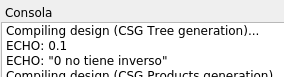
\includegraphics[width=.65\textwidth]{imagenes/consola-echo-inversa}
  \caption{Empleo del operador ternario `\lstinline!? :!'.}
  \label{fig:consola-echo-inversa}
\end{figure}
  


Antonia tomo aire, como cada vez que se veía ante la perspectiva de
tener que ofrecer una larga explicación:

---La idea es ésta: el operador `\lstinline!? :!' espera tres
expresiones. La primera debe adoptar la forma de una condición (en el
último ejemplo, se trata de \lstinline!(x==0)!). Si la condición es
verdadera, el operador devuelve el valor de la segunda expresión (el
texto \lstinline!"0 no tiene inverso"! en nuestro ejemplo); en caso
contrario, devuelve el valor de la tercera expresión
(\lstinline!(1/x)! en nuestro caso).

---¿Es como un \lstinline!if!/\lstinline!else!, pero para funciones?
---pre\-gun\-tó Cecilia, más por decir algo que para confirmar que había
entendido, cosa de la que no estaba tan segura.

---¡Exacto! ---exclamó Antonia con entusiasmo, queriendo creer que su
explicación había sido eficaz---. Te comento que los paréntesis en
cada expresión no son necesarios, salvo cuando se imponen para
resolver alguna ambigüedad. El ejemplo anterior podría haberse escrito
tranquilamente así:

\begin{lstlisting}[numbers=none]
function inversa(x)= x==0 ? "0 no tiene inverso" : 1/x;
\end{lstlisting}

\guillemotright ¡Ah! Una cosa importante ---Antonia sobreactuó como
era su costumbre al comentar los detalles finales de una novedad---:
Las dos últimas expresiones pueden ser de cualquier tipo, con tal que
representen un valor: un número, un texto entre comillas, un vector,
una matriz, etc.; cualquier cosa que vos puedas asignar a una
variable.

Cecilia volvió ahora sus ojos a la definición de la función
\lstinline!alfa(hora)!. No le pareció tan difícil de entender,
finalmente: el operador ternario primero indagaba la veracidad de la
expresión \lstinline!hemisferio=="sur"!. Si era verdadera, devolvía el
valor de la función \lstinline!alfa_sur(hora)!; en caso contrario,
retornaba el de \lstinline!alfa_norte(hora)!. Sonaba bien, pero ahora
fue ella quien quiso comprobar su funcionamiento:

\begin{lstlisting}
hemisferio="sur";
for(h=[6:3:18])
  echo(h,alfa(h));
\end{lstlisting}

\begin{figure}[ht]
  \centering
  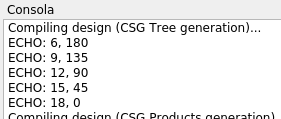
\includegraphics[width=.55\textwidth]{imagenes/consola-echo-alfa-sur}
  \caption[$alpha$ para el hemisferio sur.]{Calculo del ángulo
    $\alpha$ para el hemisferio sur.}
  \label{fig:consola-echo-alfa-sur}
\end{figure}

\begin{lstlisting}
hemisferio="norte";
for(h=[6:3:18])
  echo(h,alfa(h));
\end{lstlisting}

\begin{figure}[ht]
  \centering
  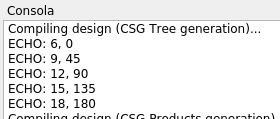
\includegraphics[width=.55\textwidth]{imagenes/consola-echo-alfa-norte}
  \caption[$alpha$ para el hemisferio norte.]{Calculo del ángulo
    $\alpha$ para el hemisferio norte.}
  \label{fig:consola-echo-alfa-norte}
\end{figure}

Parecía que la función funcionaba.

\section{Una antigua función}

Cecilia contemplaba feliz las funciones conquistadas, sin saber si
adjudicar esa felicidad al sentido estético de tan altas
construcciones sintácticas o al presentimiento de que al fin estaban
más cerca de lograr su tan ansiado reloj de Sol digital. Pero en medio
de su dicha, sintió que se colaba cierta sensación de nostalgia: una
especie de recuerdo difuso de algo que no había cerrado por
completo.

---¡Antonia! ---exclamó de repente---. Esta construcción de una
función, junto con los signos `\lstinline!?!' y `\lstinline!:!' ya la
vimos, ¿no? ---y dirigió a su amiga una mirada en la que brillaba un
pedido de ayuda.

---Claro ---dijo suavemente Antonia, con una amplia son\-ri\-sa---. ¡Qué
memoria! Pensé que te habrías olvidado. Fue hace mucho, en el capítulo
\ref{sec:analisis-literario-ii}:

\begin{lstlisting}
radio=16;
factor=1.2;

function z(i,acc=0) =
 (i==0) 
   ? radio*acc 
   : z(i-1,acc=acc+(factor+1)/pow(factor,i));
\end{lstlisting}

Cecilia sintió que un relámpago cruzaba su mente:

---¡Sí!  ¡Ahora lo recuerdo bien! Era la solución que casi no me
mostrás en ese momento... ---confirmó, devolviendo a Antonia la
sonrisa y rememorando ese ya viejo capítulo---. <<¡Cuánto avanzamos
desde entonces..!>> ---pensó, con una suave melancolía.

Cecilia recorrió ahora el texto con la seguridad que le infundía su
nueva conquista de las funciones y sus condicionales: En primer lugar,
se verificaba si \lstinline!i! era nulo en la línea 5. En caso
afirmativo, se devolvía el producto de \lstinline!radio! y
\lstinline!acc!. En caso contrario... Cecilia detuvo su lectura con
estupor. <<¡Eh!  ¡Qué es eso!>> ---pensó con alarmada
perplejidad---. <<¿En caso negativo debe devolverse el valor de la
propia función \lstinline!z!? ¡Pero si estamos dentro de la función
\lstinline!z!!>>.

El gesto de Cecilia debió haber sido lo suficientemente elocuente por
sí mismo, ya que Antonia se sintió obligada a intervenir:

---Se trata de un caso muy usual en este género literario: es un
ejemplo de \emph{recursividad}. La recursividad es muy común también
en ese otro gran género literario, tan emparentado con la
programación: la matemática. Recordemos, por ejemplo, la definición
más difundida de la función factorial:

\begin{equation*}
  n! = 
  \begin{cases}
      1 &\quad \text{si } n=1,\\
      n\times(n-1)!&\quad \text{si } n>1.
  \end{cases}
\end{equation*}


Cecilia, por supuesto, recordaba esa definición, la cual tenía un
sentido muy claro: el cálculo de $5!$, por ejemplo, podía pensarse
así: como $5>1$, $5!=5\times4!$. Pero $4!=4\times3!$, así que
$5!=5\times4\times3!$. Y así siguiendo, se llegaba hasta
$5!=5\times4\times3\times2\times1$, puesto que $1!=1$, y el descenso a
través de los números naturales allí se detenía.

---Esa definición puede escribirse de manera casi literal en
\openscad{} ---aseguró Antonia:

\begin{lstlisting}[numbers=none]
function factorial(n)= n==1 ? 1 : n*factorial(n-1);
\end{lstlisting}

\guillemotright Si \lstinline!n==1!, devuelve el valor 1; en caso
contrario, devuelve el producto \lstinline!n*factorial(n-1)!.  Parece
magia... pero funciona ---prometió Antonia, mientras escribía la
necesaria comprobación:

\begin{lstlisting}
for(i=[1:10])
  echo(i,factorial(i));
\end{lstlisting}

\begin{figure}[ht]
  \centering
  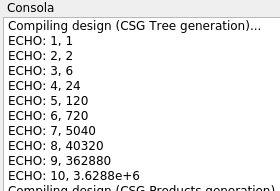
\includegraphics[width=.55\textwidth]{imagenes/consola-echo-factorial}
  \caption{Antonia demuestra el funcionamiento de una definición
    recursiva de la función factorial.}
  \label{fig:consola-echo-factorial}
\end{figure}
  
Cecilia, frente al resultado ofrecido por la figura
\ref{fig:consola-echo-factorial}, se encontró fascinada con las
posibilidades expresivas que este nuevo misterio le ofrecía; decidió,
como con tantas otras novedades conceptuales, dedicarle la escritura
de varios ejemplos a fin de conquistarlo plenamente.

---Un detalle importantísimo que nunca debés olvidar ---ad\-vir\-tió
Antonia con gesto adusto--- es el establecimiento claro del caso base;
en la definición de factorial, se trata de \lstinline!i==1!. Si ese
caso no se alcanzara nunca, la recursión no se detendría jamás. Bueno,
en realidad en \openscad{} hay un límite interno impuesto a toda
función recursiva, así que tampoco vas a romper nada. Pero en otros
lenguajes de programación podrías colgar la computadora.

Cecilia pensó que de todas formas eso ocurría casi todos los días con
las computadoras de Havard, sin necesidad de escribir funciones
recursivas con errores. Pero aceptó el consejo de Antonia como
razonable.

---Si ahora volvemos a la definición de la función \lstinline!z!,
verás que se adecua fielmente a la expresión matemáticamente clásica:
\begin{equation*}
  z(i,acc) = 
  \begin{cases}
      radio\times acc &\quad \text{si } i=0,\\
      z\left(i-1,acc+\frac{factor+1}{factor^i}\right)&\quad \text{si } i>0.
  \end{cases}
\end{equation*}

\guillemotright que a su vez es la fiel expresión recurrente de esta otra:

\[
  z(i)=radio \times
  \left[0+\frac{k+1}{k^1}+\frac{k+1}{k^2}+\frac{k+1}{k^3}+\cdots+\frac{k+1}{k^i}\right]
\]

\guillemotright En la que reemplacé `$factor$' por `$k$' para que
resultara más legible ---y Antonia se recostó contra el respaldo de su
silla, mirando su texto como una artista que contemplara el efecto
general logrado por su última pincelada sobre un retrato que, como
todos, no era otra cosa que un autorretrato.\footnote{Aún podría
  extraerse $k+1$ como factor común. (Nota del
  Editor)}$^,$\footnote{¡Pesado! (Nota de Antonia, Cecilia y Luis)}

% \subsection{Serie de Fibonacci}

% \emph{``Bien mirado, el operador ternario \lstinline! ? : ! puede
%   tomarse como un valor en sí mismo; por esta razón, puede tomar el
%   lugar de la segunda o tercera expresión de otro operador del mismo
%   tipo.''} ---agregó Antonia, y Cecilia no estaba segura de querer
% participar de lo que veía venir--- \emph{``Recordarás sin duda la
%   definición clásica de la serie de Fibonacci:''}
% \begin{equation*}
%   Fib(i)=
%   \begin{cases}
%     1&\quad \text{si } i=0 \text{ o } i=1,
%     Fib(n-2)+(F
%   \end{cases}
% \end{equation*}






%%% Local Variables:
%%% mode: latex
%%% TeX-master: "../libro"
%%% End:
